\documentclass[10pt]{article}
\usepackage[margin=1in]{geometry}
\usepackage[T1]{fontenc}
\usepackage{lmodern}
\usepackage{amsmath,graphicx,booktabs}
\usepackage[round]{natbib}
\usepackage{hyperref}
\newcommand{\model}{\textsc{TabScale}}

\title{Scaling Laws for Tabular Foundation Models}
\author{Anonymous}
\date{}

\begin{document}
\maketitle

\section{Introduction}\label{sec:intro}
We study how a tabular foundation model scales with parameters and pretraining
tables. \model{} follows residual designs \citep{he2016resnet} trained with Adam
\citep{kingma2015adam}. Our evaluation protocol is described in Section~\ref{sec:protocol}
and the scaling curve is shown in Figure~\ref{fig:scaling}.

\begin{figure}[t]
  \centering
  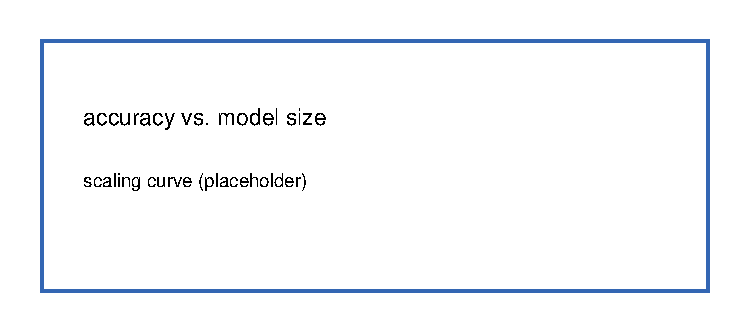
\includegraphics[width=.9\linewidth]{figures/scaling}
  \caption{Accuracy against model size.}
  \label{fig:scaling}
\end{figure}

\section{Results}\label{sec:results}
\begin{table}[t]
  \caption{Benchmark results.}\label{tab:results}
  \centering
  \begin{tabular}{@{}lccc@{}}
  \toprule
  Model & Mean OpenML-CC18 test accuracy averaged over all seventy-two classification datasets and ten seeds & AUC & Rank \\
  \midrule
  Gradient boosting & .842 & .901 & 2.1 \\
  \model{} & .861 & .913 & 1.4 \\
  \bottomrule
  \end{tabular}
\end{table}

TODO: add the compute budget sentence. Results follow the setup of \citet{grinsztajn2022tree}.

\section{Conclusion}
\model{} improves with scale.\label{mainend}

\bibliographystyle{plainnat}
\bibliography{refs}
\end{document}
